\documentclass[10pt,a4paper,titlepage]{report}
\usepackage[utf8]{inputenc}
\usepackage[spanish]{babel}
\usepackage{amsmath}
\usepackage{amsfonts}
\usepackage{amssymb}
\usepackage{float}
\usepackage{graphicx}
\usepackage{caption}
\captionsetup[table]{name=Tabla}

\usepackage{subcaption}
\usepackage{listings}

%\usepackage{listingsutf8}
\usepackage{xcolor}
\usepackage{pdfpages} %para abrir documentos en PDF
\usepackage{xr} %Para referenciar etiquetas desde otros ficheros
\usepackage{underscore} %Para que lea bien el código
\usepackage{hyperref}% Para que el índice tenga hipervínculos
\usepackage[left=2cm,right=2cm,top=2cm,bottom=2cm]{geometry}
\lstdefinestyle{customc}{
  belowcaptionskip=1\baselineskip,
  breaklines=true,
  frame=L,
  xleftmargin=\parindent,
  language=C,
  showstringspaces=false,
  basicstyle=\footnotesize\ttfamily,
  keywordstyle=\bfseries\color{green!40!black},
  commentstyle=\itshape\color{purple!40!black},
  identifierstyle=\color{blue},
  stringstyle=\color{orange},
}

\lstset{style=customc,literate=
  {á}{{\'a}}1 {é}{{\'e}}1 {í}{{\'i}}1 {ó}{{\'o}}1 {ú}{{\'u}}1
  {Á}{{\'A}}1 {É}{{\'E}}1 {Í}{{\'I}}1 {Ó}{{\'O}}1 {Ú}{{\'U}}1
  {à}{{\`a}}1 {è}{{\`e}}1 {ì}{{\`i}}1 {ò}{{\`o}}1 {ù}{{\`u}}1
  {À}{{\`A}}1 {È}{{\'E}}1 {Ì}{{\`I}}1 {Ò}{{\`O}}1 {Ù}{{\`U}}1
  {ä}{{\"a}}1 {ë}{{\"e}}1 {ï}{{\"i}}1 {ö}{{\"o}}1 {ü}{{\"u}}1
  {Ä}{{\"A}}1 {Ë}{{\"E}}1 {Ï}{{\"I}}1 {Ö}{{\"O}}1 {Ü}{{\"U}}1
  {â}{{\^a}}1 {ê}{{\^e}}1 {î}{{\^i}}1 {ô}{{\^o}}1 {û}{{\^u}}1
  {Â}{{\^A}}1 {Ê}{{\^E}}1 {Î}{{\^I}}1 {Ô}{{\^O}}1 {Û}{{\^U}}1
  {ã}{{\~a}}1 {ẽ}{{\~e}}1 {ĩ}{{\~i}}1 {õ}{{\~o}}1 {ũ}{{\~u}}1
  {Ã}{{\~A}}1 {Ẽ}{{\~E}}1 {Ĩ}{{\~I}}1 {Õ}{{\~O}}1 {Ũ}{{\~U}}1
  {œ}{{\oe}}1 {Œ}{{\OE}}1 {æ}{{\ae}}1 {Æ}{{\AE}}1 {ß}{{\ss}}1
  {ű}{{\H{u}}}1 {Ű}{{\H{U}}}1 {ő}{{\H{o}}}1 {Ő}{{\H{O}}}1
  {ç}{{\c c}}1 {Ç}{{\c C}}1 {ø}{{\o}}1 {å}{{\r a}}1 {Å}{{\r A}}1
  {€}{{\euro}}1 {£}{{\pounds}}1 {«}{{\guillemotleft}}1
  {»}{{\guillemotright}}1 {ñ}{{\~n}}1 {Ñ}{{\~N}}1 {¿}{{?`}}1 {¡}{{!`}}1 }

\title{

\includegraphics[width=0.75\textwidth]{../OdiTech Logo.pdf}  \\
\vspace*{1in}
\textbf{Informe Técnico - Económico}\\
\vspace*{0.5in}
\textbf{Taller de Proyectos II}}

\author{Autores:\\
Inés Varona Peña, David Manso Fernández, Óscar Martín Casares y Daniel Sirgo Rodríguez\\
		\vspace*{0.5in} \\
        \textbf{Universidad de Valladolid}\\
        Valladolid, España
       } \date{\today}

\begin{document}
\maketitle
\tableofcontents
\listoffigures
%\listoftables

\chapter{Resumen}
\chapter{Planteamiento inicial}
La empresa para la que trabajamos ha sido adjudicataria de un contrato con el objetivo de desarrollar un servicio de vehículo conectado consistente en el envío de información de video desde el vehículo a un servidor en el cloud. El video será procesado en el cloud para la detección automática, mediante técnicas de inteligencia artificial, de señales de tráfico en la carretera.\\

El objetivo de este proyecto es desarrollar una infraestructura de red 4G que permita la transmisión de video desde los vehículos conectados al servidor en el cloud. Esta infraestructura permitirá a la empresa ofrecer un servicio de predicción de señales de tráfico en la carretera, lo que ayudará a mejorar la seguridad y la eficiencia en el tráfico. Esto se logrará desarrollando un demostrador previo al despliegue de la red para probar la capacidad de la empresa para desplegar el servicio, y presentando una memoria técnicoeconómica que detalle el despliegue de la red en el tramo de autovía A-62 desde el kilómetro 158 hasta el kilómetro 231. Además, la empresa tendrá que demostrar contar con los permisos legales pertinentes para el despliegue del servicio, que tendrá una duración máxima de 6 meses.

\chapter{Solución}
\chapter{Normativa}
\chapter{Costes}

\chapter{Anexo I}
\chapter{Anexo II}
\chapter{Anexo III}
\section{Objetivos}

\section{Metodología del proyecto}
Metodologia del proyecto

\section{Arquitectura}
\section{Infraestructura de la red}
Para el proceso de creación de la red 4G, se usó el \textit{software} srsRAN, una implementación de código abierto de una red de acceso radio (RAN) que utiliza \textit{hardware} SDR. En nuestro caso, se ha utilizado una BladeRF 2.0 micro xA9 de Nuand con dos canales rx y tx MIMO.

Para ello, se siguieron los siguientes pasos:


\begin{enumerate}
\item Descarga de la última versión de \textbf{Ubuntu}, \textbf{22.04 LTS}.
\item Grabación de la ISO en un pincho a través de \textbf{UNetbootin} y posterior instalación de Linux en un ordenador sin sistema operativo (proporcionado por la empresa).
\item Instalación de los drivers de la \textit{Blade} siguiendo el manual de \textit{GitHub}:\\
 \url{https://github.com/Nuand/bladeRF/wiki/Getting-Started:-Linux}

\begin{lstlisting}
sudo add-apt-repository ppa:nuandllc/bladerf
sudo apt-get update
sudo apt-get install bladerf
\end{lstlisting}

\item Conexión de la Blade: Las antenas se deben conectar en los puertos tx1 y rx1 (configuración por defecto, sin embargo se podrían conectar a tx2 y rx2 haciendo los cambios correspondientes en los ficheros de configuración) con un grado de 90º entre ellas para evitar el efecto de \textit{crosstalk}, como se muestra en la figura \ref{blade}. La Blade se debe conectar a un puerto USB 3.0 que presente el ordenador ya que en un puerto USB 2.0 no se detectaría correctamente.\\

\begin{figure}[H]
	\centering
	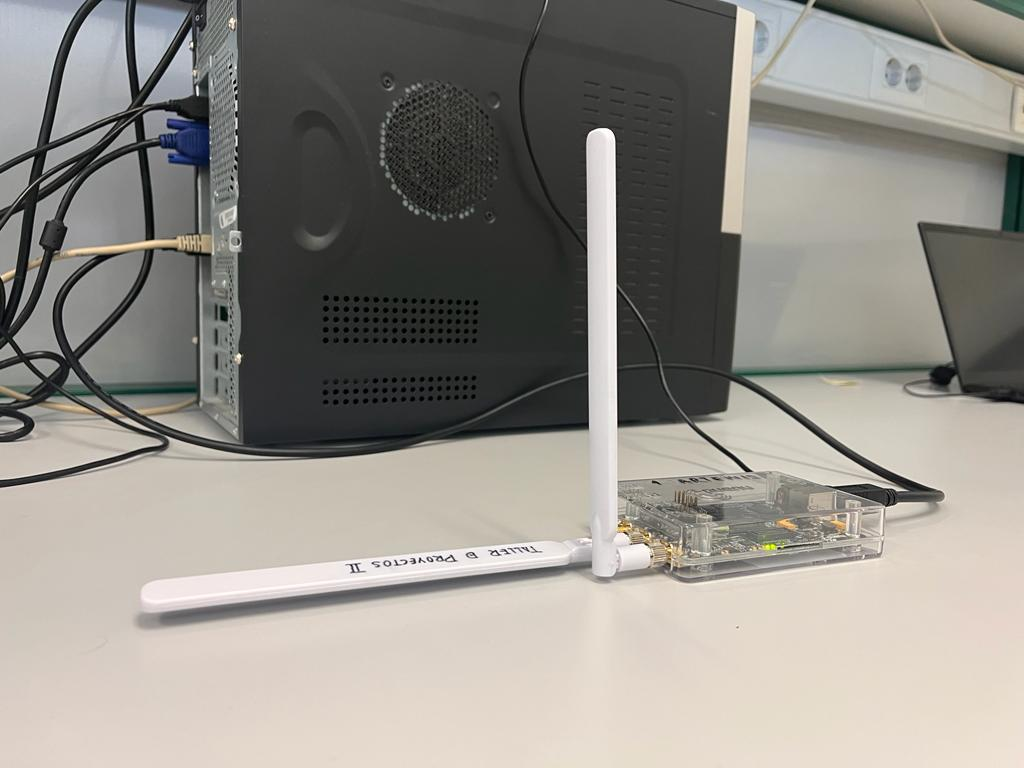
\includegraphics[width=\textwidth]{Imagenes/AnexoI_Manual/RED/blade.jpeg}
	\caption{Dataset descargado con los ficheros TXT}
	\label{blade}
\end{figure}

\item Instalación de \textbf{srsran} siguiendo el manual de GitHub y las librerías \textbf{boost} y \textbf{libboost}:\\
\url{https://docs.srsran.com/projects/4g/en/latest/general/source/1_installation.html}\\
\url{https://docs.srsran.com/projects/4g/en/latest/getting_started.html}

\begin{lstlisting}
git clone https://github.com/srsRAN/srsRAN_4G.git
cd srsRAN_4G
mkdir build
cd build
cmake ../
make
make test
sudo make install
srsran_4g_install_configs.sh user
\end{lstlisting}

\item Modificación de los archivos de configuración que se encuentran en la ruta \textit{root/.config/srsran/}. Los cambios se deben hacer como superusuario:
\begin{itemize}
	\item epc.conf: contiene la configuración específica de un controlador de paquetes Evolved Packet Core (EPC) en una arquitectura de red LTE 
	\item enb.conf: cotiene la configuración específica de un nodo de banda base (eNodeB).
	\item user_db.csv: que contiene una base de datos de usuarios en formato tabular.
\end{itemize}

En el archivo \textbf{enb.conf} se cambiaron los valores de \textbf{MCC} y \textbf{MNC} que están disponibles en las hojas de datos de las SIMs (y en la propia tarjeta SIM), y se establecieron sus valores correspondientes (\textbf{901-70}) para que correspondan con el IMSI. También se modificó el valor de la frecuencia central. cambiando el valor de \textbf{dl_earfcn}, para ello se utilizó \cite{earn}, estableciéndolo este valor 3050, lo que corresponde a un valor de frecuencia central \textit{downlink} de 2650.  Por último, se estableció el ancho de banda en 5MHz cambiando el valor de \textbf{n_prb} a \textbf{25}. Para mejorar el alcance de la red, se aumentó la ganancia de transmisor, cambiando el valor de \textbf{tx_gain} a 90.

En el archivo \textbf{epc.conf} se modificaron los valores de \textbf{MCC} y \textbf{MNC} (igual que en el caso anterior) y se añadieron los nombres de la red con:
\begin{lstlisting}
    full_net_name= NOMBRE
    short_net_name= NOMBRE
\end{lstlisting}

En el archivo \textbf{user_db.csv} se creó un usuario nuevo con la siguiente información:
\begin{lstlisting}
    nombre, mil (Auth), IMSI (aparece en las hojas de las sims),
    KEY (aparece en las hojas de las sims), opc,
    OPC(aparece en las hojas de las sims), 9000,
    sqn (poner todo a ceros, aunque cada vez que se levanta la red cambia automáticamente),
    7 (QCI), dynamic (IP_alloc)
\end{lstlisting}

\item Ahora que tenemos conectividad entre el enb y el epc, necesitamos que estos la tengan para el exterior, por lo que necesitamos configurar el ordenador (que ejecuta el núcleo) para que reencamine los paquetes a través de la interfaz de red. Para eso ejecutamos el siguiente comando.

\begin{lstlisting}
    srepc_if_masq.sh enp0s25
\end{lstlisting}

\item Una vez está la red configurada, es hora de levantarla, ejecutamos:
\begin{lstlisting}
    srsepc epc.conf
    srsenb enb.conf
\end{lstlisting}

\item Una vez obtenida la conexión a internet con la red 4G, nos bajamos los ficheros \textit{python} de control del coche para crear el servidor \textit{cloud} e instalamos el servidor \textbf{MQTT Mosquitto}, diseñado para facilitar la comunicación entre dispositivos (en nuestro caso la SDR y el coche) itercambiando mensajes MQTT. Este servidor facilita la integración del proyecto, facilitando el monitoreo y control remoto del coche durante su funcionamiento.
Para su instalación en el ordenador (que actuará como servidor), se ejecutan los siguientes comandos:

\begin{lstlisting}
	sudo apt-get update
	sudo apt-get install mosquitto
\end{lstlisting}

\item Modificamos el fichero de configuración /etc/mosquitto/mosquitto.conf con las siguientes líneas:
\begin{lstlisting}
	persistence true
	persistence_location /var/lib/mosquitto/
	allow_anonymous true
	listener 1883 10.0.128.176
	bind_interface enp0s25
	log_type information
	log_type warning
	log_type error
\end{lstlisting}

\item Una vez configurados los ficheros, reiniciamos el servicio mosquitto para que se apliquen los cambios:
\begin{lstlisting}
	sudo systemctl restart mosquitto
\end{lstlisting}

\item Para instalar el servicio en el móvil (que actuará como cliente) usamos la aplicación MyMQTT. Para comprobar el tránsito de mensajes que el coche envía nos suscribimos a los tópicos básicos que se especifican en el manual de usuario del coche. Para ello, habrá que poner el ID del vehículo y el tópico al que nos queramos suscribir (Ver figura \ref{fig:mosq1}). Si la comunicación es exitosa, se debería observar algo similar a la imagen \ref{fig:mosq3}:

 \begin{figure}[H]
    \centering
    \subfloat[Suscripciones a los tópicos desde el móvil\label{fig:mosq1}]{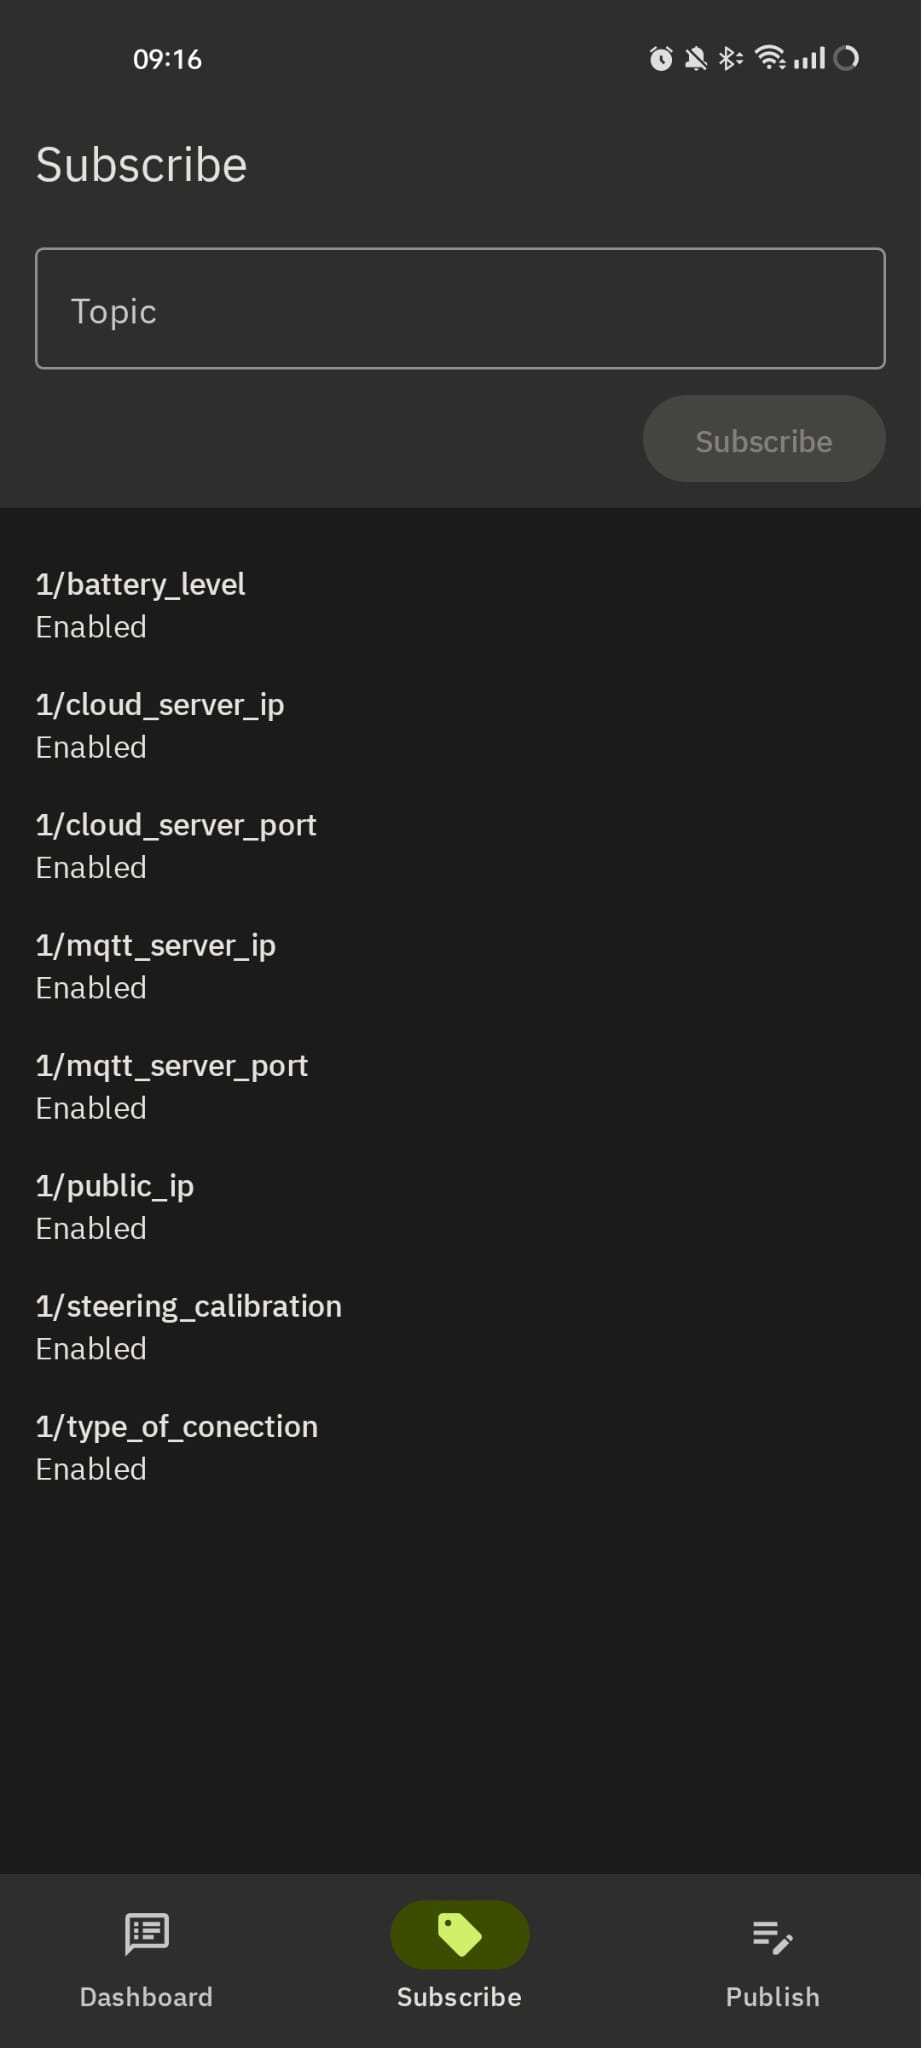
\includegraphics[width=0.4\textwidth]{Imagenes/Rendimiento/mosquitto1.jpeg}}
    \hspace{0.5cm}
    \subfloat[Información mostrada al iniciar la conexión\label{fig:mosq3}]{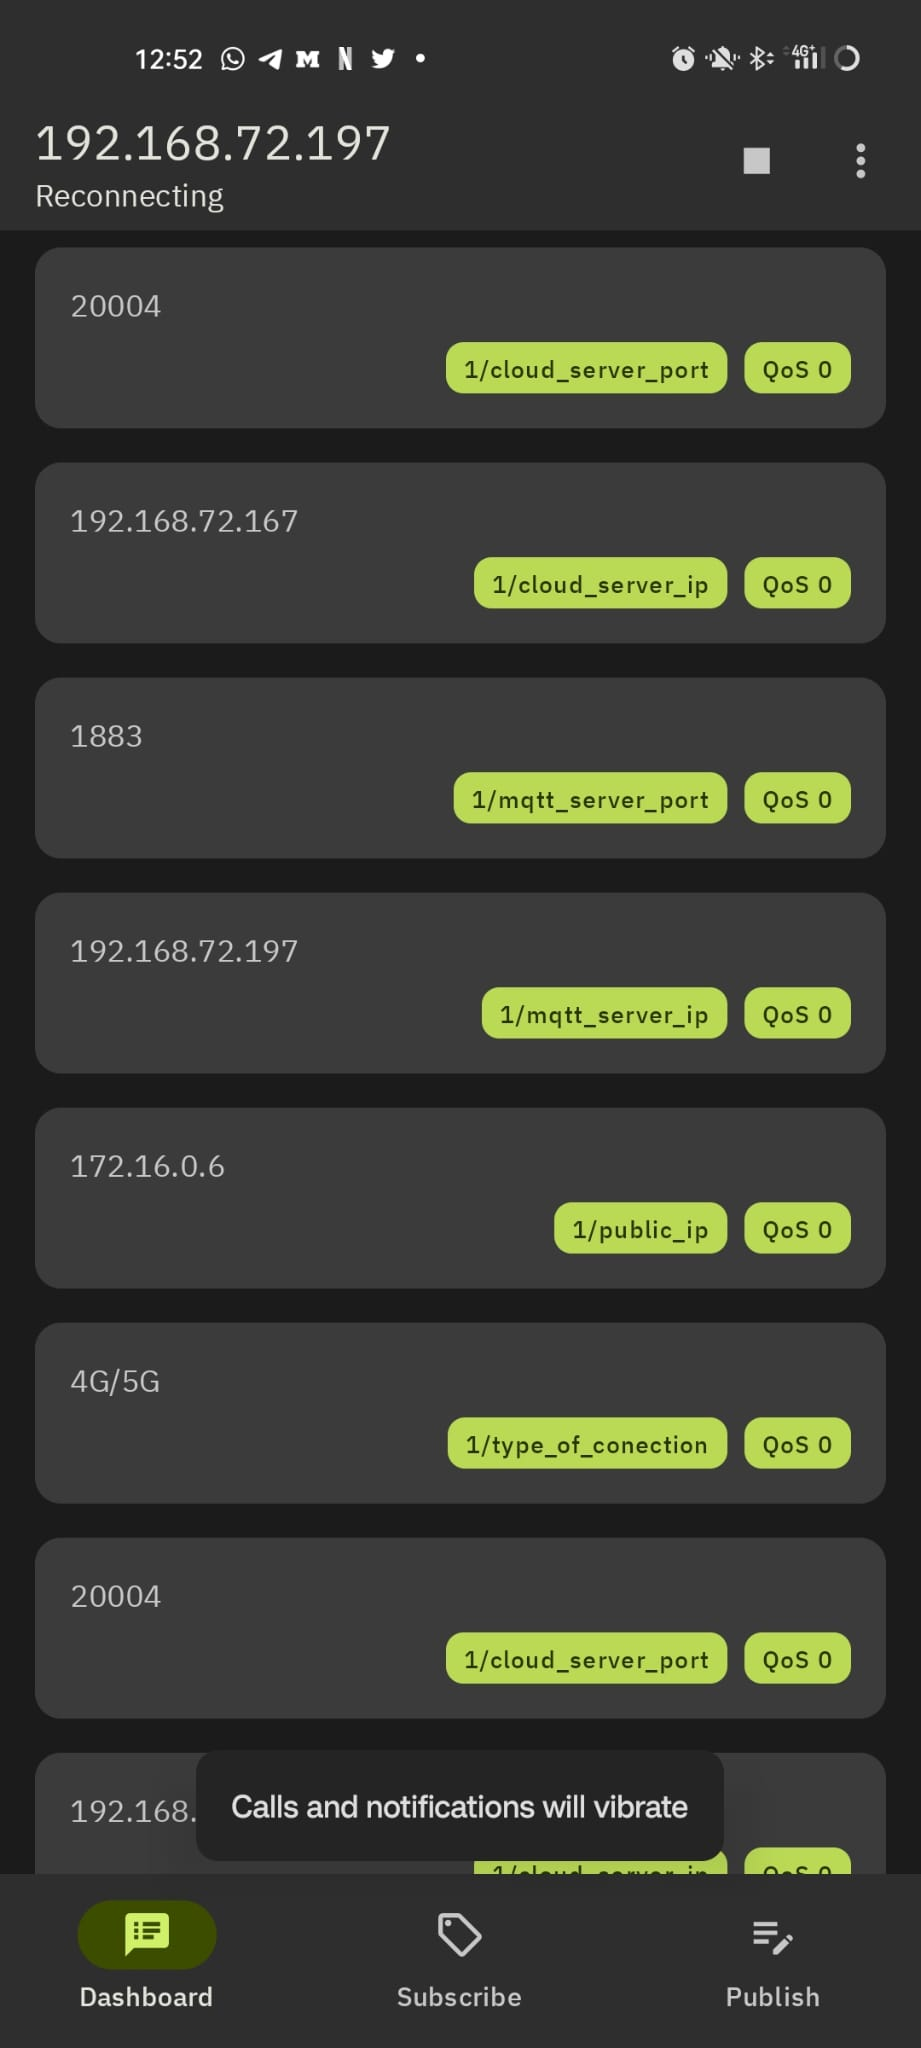
\includegraphics[width=0.4\textwidth]{Imagenes/Rendimiento/mosquitto3.jpeg}}
    \caption{Capturas de pantalla de la aplicación móvil MyMQTT para cliente suscrito}
\end{figure}


\item Tras configurar tanto el servidor como el cliente mosquitto, lanzamos el servicio y comprobamos su estado usando los comandos:
\begin{lstlisting}
	sudo systemctl start mosquitto
	sudo systemctl status mosquitto
\end{lstlisting}


\item Para comunicarnos con el coche, publicaremos los tópicos que se indican en el manual de configuración del coche, como podemos ver en la imagen \ref{mosquitto2}:

 \begin{figure}[H]
    \centering
    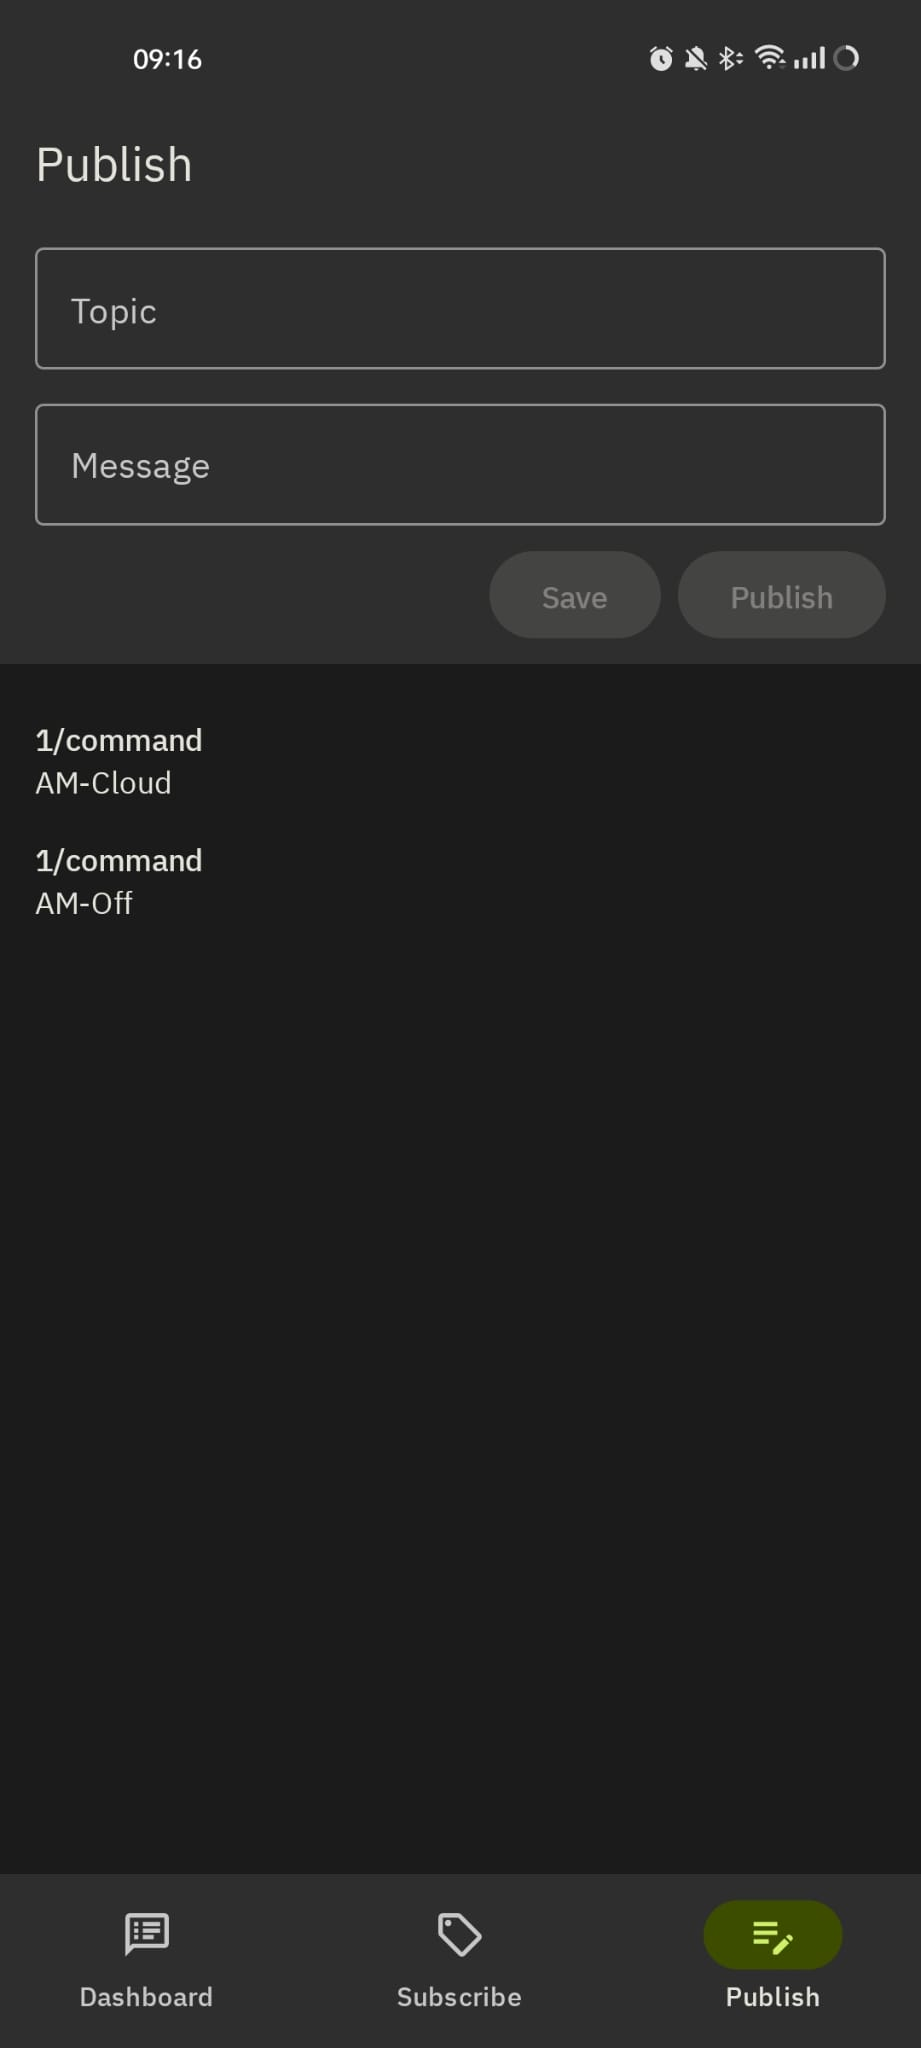
\includegraphics[width=0.35\textwidth]{Imagenes/Rendimiento/mosquitto2.jpeg}
    \caption{Publicación de comandos desde el móvil}
    \label{mosquitto2}
\end{figure}

\end{enumerate}

\section{Identificación de imágenes}
\chapter{Normativa}

\chapter{Informe técnico de empresa}
\section{Valoración económica}
\section{Conclusiones y líneas futuras}

\chapter{Referencias}

\end{document}